\documentclass{article}
\usepackage[utf8]{inputenc}
\usepackage{amsfonts}
\usepackage{amsmath}
\usepackage{graphicx}
\usepackage[a4paper, total={6in, 8in}]{geometry}
\usepackage{setspace}

\newcommand\tab[1][1cm]{\hspace*{#1}}
\onehalfspacing
\author{Frederic Becerril}

\begin{document}

\part*{Chapitre 1: Produit scalaire et orthogonalité}

\section{Produit scalaire dans le plan}

\subsection{Le plan vectoriel}

Pour mémoire le plan vectoriel est l'ensemble des vecteurs du plan.
Un vecteur $\vec{u}$ correspond à une translation et est caractérisé
par une direction, un sens, une longueur qu'on note $||\vec{u}||$
(norme de $\vec{u}$)

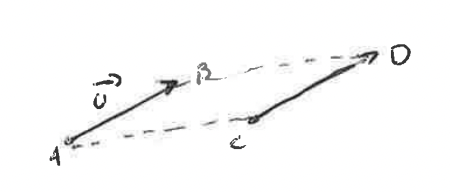
\includegraphics{images/image01.png}

$\vec{u} = \overrightarrow{AB} = \overrightarrow{CD}$ \newline
$\overrightarrow{AB} = \overrightarrow{CD} \Leftrightarrow$ (ABCD) parrallélogramme

C'est l'exemple le plus simple et quelque part le plus fondamental d'ev (on peut "voir") qu'on note $\overrightarrow{\widehat{O}}$

\begin{itemize}

    \item $\vec{0} \in \overrightarrow{\widehat{O}}$
    \item Multiplication par scalaire 
\end{itemize}
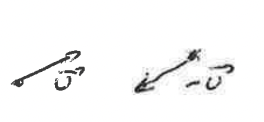
\includegraphics{images/image03_1.png}
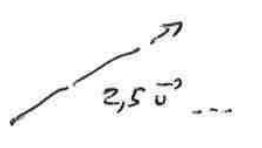
\includegraphics{images/image03_2.png}
\begin{itemize}
    \item Somme $\vec{u} \neq \vec{v}$:
\end{itemize}

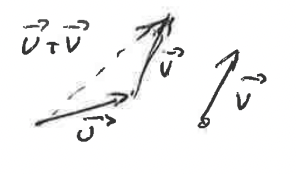
\includegraphics{images/image04.png}

\paragraph{Remarque 1:}
$||\vec{u} + \vec{v}|| \leq ||\vec{u}|| + ||\vec{v}||$
(Inégalité triangulaire)
\paragraph{Remarque 2:}
Si $\vec{u}$ et $\vec{v}$ sont non nuls et orthogonaux (i.e. directions perpendiculaire);

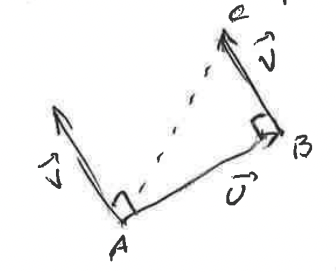
\includegraphics{images/image02.png}

Alors $||\vec{u} + \vec{v}||^2 = ||\vec{u}||^2 + ||\vec{v}||^2$
et reciproquement.

\subsection{Produit scalaire}

\paragraph{Définition:}

Pour tous vecteurs $\vec{u}$, $\vec{v}$ on définit leur produit scalaire par: \\
$\vec{u} . \vec{v} = \frac{1}{2} (||\vec{u} + \vec{v}||^2 - ||\vec{u}||^2 - ||\vec{v}||^2) \in \mathbb{R}$

Ce produit défini une application $\overrightarrow{\widehat{O}} x \overrightarrow{\widehat{O}} = \overrightarrow{\widehat{O}}^2 \rightarrow \mathbb{R}$
(Qu'on appelle aussi \underline{forme} car à valeur dans $\mathbb{R}$)
notée $<\vec{u}|\vec{v}>$ où plus $f(\vec{u}, \vec{v})$ comme une fonction.

\paragraph{Remarque:}

\begin{itemize}
    \item $\forall (\vec{u}, \vec{v}) \in \overrightarrow{\widehat{O}} \tab \vec{u}, \vec{v} orthogonaux \Leftrightarrow \vec{u} . \vec{v} = 0$
    \item $\vec{v} . \vec{0} = \vec{0} . \vec{v} = 0$ (Tt vecteur est orthogonal au vecteur $\vec{0}$)
    \item $\vec{u} . \vec{v} = 0 \Leftrightarrow ||\vec{u} + \vec{v}||^2 = ||\vec{u}||^2 + ||\vec{v}||^2 \tab | \tab \vec{u} . \vec{u} = \vec{u}^2 = ||\vec{u}||^2$
\end{itemize}

\subsection{Repère et base orthonormé}

Dans le plan, si on se donne un repère orthonormé (O, I, J) a une base orthonormé du plan vectoriel = \{$\vec{i} = \overrightarrow{OI}, \vec{j} = \overrightarrow{OJ}$\}

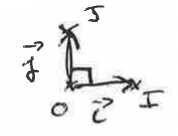
\includegraphics{images/image05.png} $||\vec{i}|| = ||\vec{j}|| = 1 \tab et \tab \vec{i} . \vec{j} = 0$
$$
\mbox{Et tout vecteur} \vec{u} \mbox{ s'indetifie à un couple de réels}
\left( 
    \begin{array}{c}
    x_1 \\
    x_2 \\
    \end{array}
\right)
\mbox{ de } \mathbb{R} \times \mathbb{R} = \mathbb{R}^2
$$
$\mbox{et } ||\vec{u}|| = \sqrt{x^2 + y^2}$

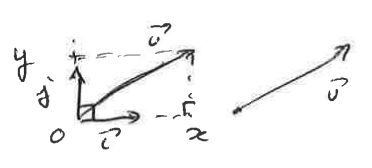
\includegraphics{images/image06.png}

\paragraph{Remarque:}

Il y a ambiguité matriciellement entre
$$
\left( 
    \begin{array}{c}
    x_1,
    x_2
    \end{array}
\right) \in M_{1, 2}(\mathbb{R}) \mbox{ et}
\left( 
    \begin{array}{c}
    x_1 \\
    x_2 \\
    \end{array}
\right) \in M_{2, 1}(\mathbb{R})
$$
On adopte pour $\mathbb{R}^2, \mathbb{R}^n$ et leurs vecteurs la notation verticale. \\
$\mathbb{R}^n = M_{n, 1}(\mathbb{R})$
$$
\vec{x} = 
\left( 
    \begin{array}{c}
    x_1 \\
    \vdots \\
    x_n \\
    \end{array}
\right)
$$
et 
$$
\vec{x}^T =
\left( 
    \begin{array}{c}
    x_1,
    \dots,
    x_n
    \end{array}
\right)
$$

\paragraph{Proprieté:}

Si
$$
\vec{u} = 
\left( 
    \begin{array}{c}
        y \\
        x \\
    \end{array}
\right) = x \vec{i} + y \vec{j} 
\mbox{ et } \vec{v} = 
\left( 
    \begin{array}{c}
        y' \\
        x' \\
    \end{array}
\right)\mbox{, alors } \vec{u} . \vec{v} = xx' + yy'
$$

\paragraph{Remarque:}

$$
\vec{u} . \vec{v} = 
\begin{pmatrix}
    x, y
\end{pmatrix}
\begin{pmatrix}
    x'\\
    y'\\
\end{pmatrix}
=
\begin{pmatrix}
    x\\
    y\\
\end{pmatrix}^T
\begin{pmatrix}
    x'\\
    y'\\
\end{pmatrix}
$$
au sens des matrices !

\paragraph{Preuve:}

$$
\vec{u} + \vec{v} = 
\begin{pmatrix}
    x + x'\\
    y + y'\\
\end{pmatrix}
\mbox{ donc }
$$
$||\vec{u}||^2 = x^2 + y^2 \mbox{ et } ||\vec{v}||^2 = x'^2 + y'^2$ \\
$||\vec{u} + \vec{v}||^2 = (x + x')^2 + (y + y')^2 = x^2 + 2xx' + x'^2 + y^2 + 2yy' + y'^2$ \\
$\mbox{d'où } \vec{u} . \vec{v} = \frac{1}{2}(||\vec{u + v}||^2 - ||\vec{u}||^2 - ||\vec{v}||^2)$ \\
\tab[1.4cm]$= \frac{1}{2}(2xx' + 2yy') = xx' + yy'$

\subsection{Proprietés algébriques}

$\phi : \overrightarrow{\widehat{O}} \times \overrightarrow{\widehat{O}} \rightarrow \mathbb{R} \mbox{ est une \underline{forme}}$ \\
\tab[0.5cm]$(\vec{u}, \vec{v}) \longmapsto \vec{u} . \vec{v}$

\begin{itemize}
    \item Symétrique (S): \\
$\forall(\vec{u}, \vec{v}) \in \overrightarrow{\widehat{O}}^2 \tab \vec{u}.\vec{v} = \vec{v}.\vec{u}$

    \item Bilinéaire (B): \\
$\forall(\lambda, \mu) \in \mathbb{R}^2 \tab \forall(\vec{u}, \vec{v}, \vec{w}) \in \overrightarrow{\widehat{O}}^3$ \\
\tab $(\lambda\vec{u} + \mu\vec{v}).\vec{w} = \lambda(\vec{u}.\vec{w}) + \mu(\vec{v}.\vec{w})$ \\
\tab $\vec{u}.(\lambda\vec{v} + \mu\vec{w}) = \lambda(\vec{u}.\vec{v}) + \mu(\vec{u}.\vec{w})$

    \item Definie positif (P): \\
$\forall\vec{x} \in \overrightarrow{\widehat{O}} \backslash \{\vec{0}\} \tab \vec{x}.\vec{x} > 0$
$$
\mbox{ où encore }
\left\{
    \begin{array}{ll}
        \forall\vec{x} \in \overrightarrow{\widehat{O}} \tab \vec{x}.\vec{x} \geq 0 \\
        \vec{x}.\vec{x} = \vec{0} \Leftrightarrow \vec{x} = \vec{0}
    \end{array}
\right.
$$

\end{itemize}

\paragraph{Remarque:}

La symétrie simplifie la bilinéarité. \\
Si $\vec{x} = \vec{0} \tab \vec{x}.\vec{x} = \vec{0} \mbox{ aussi d'après la bilinéarité}$

\subsection{Angle et produits scalaire}

Soient $\vec{u}, \vec{v}$ deux vecteurs \underline{non nuls} et $\theta = \widehat{(\vec{u},\vec{v})}$ \\
Alors $\vec{u}.\vec{v} = ||\vec{u}||.||\vec{v}||.cos(\theta)$

\paragraph{Preuve:}

On regarde les coordonnées dans la base orthonormé $\{\vec{i},\vec{j}\}$ formé de $\vec{i} = \frac{\vec{u}}{||\vec{u}||}$ et $\vec{j}$ de norme 1 tq $\widehat{(\vec{i}, \vec{j})} = \frac{\pi}{2}$

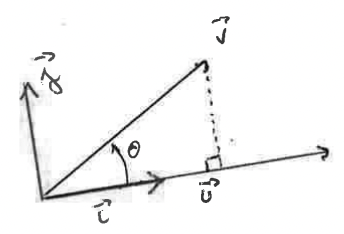
\includegraphics{images/image07.png}

$$
\vec{u} = 
\begin{pmatrix}
    ||\vec{u}||\\
    0\\
\end{pmatrix}
\tab \vec{v} = 
\begin{pmatrix}
    ||\vec{v}|| * cos(\theta)\\
    ||\vec{v}|| * sin(\theta)\\
\end{pmatrix}
$$

On en déduit ici une inégalité importante.

\paragraph{\underline{Inégalité de Cauchy-Schwarz}} \mbox{}\\
$\forall (\vec{u}, \vec{v}) \in \overrightarrow{\widehat{O}}$
$|\vec{u}.\vec{v}| \leq ||\vec{u}||.||\vec{v}||$
On a égalité si et seulement si $\vec{u} \mbox{ et } \vec{v}$ sont colinéaires.

\section{Produit scalaire dans un $\mathbb{R}$ev}

Soit E un $\mathbb{R}$ev quelconque (pas forcément de dimension finie)

\subsection{Définition}

\paragraph{Un produit scalaire sur E est une application $f:ExE\rightarrow\mathbb{R}$ qui vérifie les Proprieté (S), (B), (P) \\
C'est a dire une forme bilinéaire, défini positif et symétrique \\}

Si $(x, y) \in E^2$, ce produit scalaire peut s'écrire comme une fonction $f(x,y)$ (ou $g(x,y)$ ou autre) ou comme un produit $x.y$ ou encore $<x|y>$

Un espace E muni d'un produit scalaire est appelé un espace \underline{prehilbertien}. Si E est de dimension finie, on appelle cette espace un \underline{espace euclidien}.

\paragraph{Exemple fondamental:}

$$
\mbox{Sur } \mathbb{R}^n \mbox{ on définit pour tous }
a = 
\begin{pmatrix}
    a_1\\
    \vdots\\
    a_n\\
\end{pmatrix}
\mbox{ et b} =
\begin{pmatrix}
    b_1\\
    \vdots\\
    b_n\\
\end{pmatrix}
$$
$<a | b> = a^T . b = a_1b_1 + \dots + a_nb_n$
$= \sum_{i=1}^{n} a_ib_i$ \\
C'est un produit scalaire sur $\mathbb{R}^n$ qu'on appellera le produit scalaire usuel sur $\mathbb{R}^n$

\paragraph{\underline{Preuve à connaitre}}
\paragraph{Autres exemples} (voir exercices)
$$\mbox{Dans } \mathbb{R}^2 \tab
<
\begin{pmatrix}
    x\\
    y\\
\end{pmatrix}
|
\begin{pmatrix}
    x'\\
    y'\\
\end{pmatrix}
> = xx' + \frac{1}{2}xy' + \frac{1}{2}x'y + yy'
$$
\tab[1.4cm] $\mbox{Dans } C^0([0,1], \mathbb{R}) \tab <f|g> = \int_{0}^{1}f(t)g(t)dt$ \\
\tab[1.4cm] $\mbox{Dans } \mathbb{R}_2[X] \tab <P|Q>=P(0)Q(0) + P(1)Q(1) + P(2)Q(2)$

\subsection{Norme associée}

Dans un espace prehilbertien $(E, <|>)$ on définit la norme euclidienne associée:
$\forall x \in E \tab ||x|| = \sqrt{<x|x>}$
C'est une application de E dans $\mathbb{R}^+ (\vec{x} \longmapsto ||x||)$ qui vérifie
\begin{itemize}
    \item $\forall \lambda \in \mathbb{R} \tab[0.5cm] \forall x \in E \tab[0.5cm] ||\lambda x || = |\lambda|.||x||$
    \item $\forall x \in E \tab ||x|| = 0 \Leftrightarrow x = 0_E$
    \item $\forall(x, y) \in E^2 \tab ||x + y|| \leq ||x|| + ||y||$
\end{itemize}

Ces 3 proprietés définissent ce qu'on appelle une norme.

Le point 3 le plus délicat à montrer et se base sur l'inégalité de Cauchy-Schwarz:

\paragraph{Théorème:}

Soit $(E, <|>)$ un espace prehilbertien \\
$\forall(x, y) \in E^2 \tab |<x|y>| \leq ||x||.||y||$ et on a égalité ssi x et y sont colinéaires

\paragraph{Preuve à connaitre !:}

\begin{itemize}
    \item Si $y = 0$ alors c'est évident (on a même égalité car $<x|0_E> = 0$)
    \item Sinon on regarde, pour $t \in \mathbb{R}$ \\
$0 \leq ||x + ty||^2$ \\
$\tab = <x + ty | x + ty> = <x|x> + t<x,y> + t<y|x> + t^2 <y|y>$ \\
$\tab = ||x||^2 + 2t<x|y> + t^2 ||y||^2 = P(t)$
p un polynôme du second degré toujours positif donc \\
$\bigtriangleup = 4<x | y>^2 - 4||x||^2||y||^2 \leq 0$ \\
et $|<x | y>| \leq ||x||.||y||$
    \begin{itemize}
        \item Si x et y sont colinéaires alors $\exists t_0 \in \mathbb{R} \mbox{ tq } x = t_0 * y$ \\
et $P(-t_0) = 0$ d'où $\bigtriangleup = 0 \mbox{ et donc } |<x | y>| = ||x||.||y||$
        \item Si $|<x | y> = ||x||.||y|| \mbox{ alors } \bigtriangleup = 0 \mbox{ et } \exists \alpha \mbox{ tq } P(\alpha) = 0$ \\
donc $0 = ||x + \alpha y||^2 \mbox{ d'où } x + \alpha y = 0$ CQFD
    \end{itemize}
\end{itemize}

Grâce à cette inégalité on retrouve l'inégalité triangulaire \\
$\forall(x,y) \in E^2 ||x + y||^2 = ||x||^2 + 2<x|y> + ||y||^2$ \\
$\tab[3.3cm] \leq ||x||^2 + 2||x||.||y|| + ||y||^2 = (||x|| + ||y||)^2$

Donc $\forall(x, y) \in E^2 ||x + y|| \leq ||x|| + ||y||$

\subsection{Orthogonalité des vecteurs}

Comme dans le plan, dans $(E, <|>)$, deux vecteurs x et y sont \underline{orthogonaux} ssi $<x|y> = 0 \tab[0.5cm] x \perp y$ \\
On a de nouveau l'égalité de Pythagore: \\
$x \perp y \\Leftrightarrow ||x + y||^2 = ||x||^2 + ||y||^2$

\end{document}